\subsection{GUI}

Brugergrænsefladen gav særlige udfordringer i designfasen. Da programmet QT blev anvendt til at designe og implementer brugergrænsefladen. Udfordringerne bestod primært i at kendskabet til programmet QT ikke var særligt stort. Da QT selv skaber klasserne og metoderne er det svært at beskrive disse på forhånd. Derfor blev det besluttet at klasserne først skulle udarbejdes efter at brugergrænsefladen var designet. 

For at holde styr på den indtastede og den resterende tid er der blev oprettet en Count klasse . Denne count klasse er implementeret som en domainklasse da det er her den resterende tid for vinåbningen gemmes. Det er denne klasse som skal sørge for at tiden tælles ned når den startes. Illustrationen af countklassen kan ses på figur x.

\begin{figure}[H]
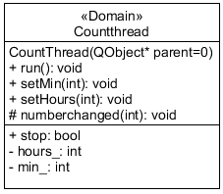
\includegraphics[scale=1]{tex/Design/GUI/Fotos/CountThread}
\caption{CountThread klasse illustreret}
\end{figure}

Der er i alt 2 klasser i brugergrænsefladen. Der er en klasse for MainWindow, hvor alle funktionerne er defineret. MainWindow er klassen som sørger for at vise den grafiske brugergrænseflade. Det er her alle trykknap funktionerne er defineret. Klassen ses illustreret på figur x. 

\begin{figure}[H]
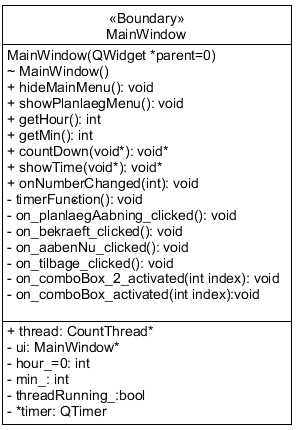
\includegraphics[scale=1]{tex/Design/GUI/Fotos/MainWindow}
\caption{MainWindow klasse illustreret}
\end{figure}

Brugergrænsefladen er state styret. Derfor har det været nødvendigt at lave et statemachine diagram for brugergrænsefladen. Der er i alt 3 overordnede states for hele system. De tre states er, ”Åbning”, ”Venter på åbning” og ”Åbning stoppet”.

Når vinåbneren er i gang med at åbne en vinflaske, så er den i staten ”Åbning”. Der er to ting der kan bringe systemet til denne state. Den første er at brugeren igennem brugergrænsefladen trykker på knappen ”Åbn nu”. Dette vil få systemet til at starte åbningen, og dermed bringe systemet i staten ”Åbning”. Den anden handling der kan bringe systemet i denne state, er når tiden under ”Planlæg åbning” menuen udløber og systemet dermed starter åbningen på vinflasken. 

Staten ”Venter på åbning” startes ved at brugeren under ”Planlæg åbning” menuen sætter en tid og trykker på bekræft. Når brugeren starter tiden, vil systemet begynde at tælle ned indtil åbningen påbegyndes. Den tid hvor systemet venter på at tiden udløber således at åbningen kan påbegyndes er staten ”Venter på åbning”.

Den sidste state er ”Åbning stoppet”. Det er denne state systemet starter ud med at være i. I denne state foretager systemet sig ingenting. Når åbningen er færdiggjort kommer systemet i denne state. Den fulde statemachine diagram kan ses i bilag x.